\documentclass{article}
\usepackage{amsmath}
\usepackage{amssymb}
\usepackage{bbm}
\usepackage[pdftex]{graphicx}
\usepackage[framed,numbered,autolinebreaks,useliterate]{mcode}
\lstset{breakatwhitespace=false}
\usepackage{pgfplots}

\pdfpagewidth 8.5in
\pdfpageheight 11in
\topmargin -1in
\headheight 0in
\headsep 0in
\textheight 8.5in
\textwidth 6.5in
\oddsidemargin 0in
\evensidemargin 0in 
\headheight 50pt
\headsep 0in
\footskip .75in

\title{STA 601 - Lab 9}
\author{Kedar Prabhudesai}
\date{November 27, 2013}

\begin{document}
\maketitle

We have an additional parameter to do inference on. Let, $W_i = 1$, denote weekday and $W_i = 0$ denote weekend. 
\begin{eqnarray*}
W_i &\sim& Bernoulli(\theta)\\
\end{eqnarray*}

If $W_i = 1,$ $X_i \sim log\mathcal{N}(\mu_1,\tau_1),$ else $X_i \sim log\mathcal{N}(\mu_2,\tau_2).$\\

\noindent {\underline{\textbf{Data Likelihood:}}}\\

Let $\tau = 1/\sigma^2,$ and $k$ is the number of weekdays. 
\begin{eqnarray*}
L(X^n,W^n \mid \mu_1,\tau_1,\mu_2,\tau_2,\theta) &=& \prod_{i=1}^{n}{\left[\mathbbm{1}(W_i = 1)log\mathcal{N}(\mu_1,\tau_1) + \mathbbm{1}(W_i = 0)log\mathcal{N}(\mu_2,\tau_2)\right]} \times \prod_{i=1}^{n}{\binom{n}{k}\theta^k(1-\theta)^{n-k}}\\
\end{eqnarray*}

\noindent {\underline{\textbf{Priors:}}}\\

We use the same priors we defined on $\mu$ and $\tau$ from last time. 

\begin{eqnarray*}
\mu_j &\sim& \mathcal{N}(\mu_{j0},\tau_{j0})
\therefore p(\mu_j) \propto exp\left[\frac{-\tau_{j0}(\mu_j-\mu_{j0})^2}{2}\right]\\
\tau_j &\sim& Gamma(\alpha_j,\beta_j)
\therefore p(\tau_j) \propto \tau_j^{\alpha_j-1}exp(-\beta_j\tau_j)\\
\theta &\sim& Beta(5,2)
\therefore p(\theta) \propto \theta^{5-1}(1-\theta)^{2-1}\\
\end{eqnarray*}

\noindent {\underline{\textbf{Posterior:}}}\\
\begin{eqnarray*}
p(\mu_1,\tau_1,\mu_2,\tau_2,\theta \mid X^n,W^n) &\propto& L(X^n,W^n \mid \mu_1,\tau_1,\mu_2,\tau_2,\theta) \times p(\mu_1) \times p(\tau_1) \times p(\mu_2) \times p(\tau_2) \times p(\theta)\\
\end{eqnarray*}

\pagebreak

\noindent {\underline{\textbf{Full Conditionals:}}}\\
\begin{eqnarray*}
p(\theta \mid \ldots) &\propto& \theta^{5+k-1}(1-\theta)^{2+n-k-1}\\
\therefore p(\theta \mid \ldots) &\propto& Beta(5+k,2+n-k)\\
\end{eqnarray*}
-----------------------\\
\begin{eqnarray*}
p(\mu_1 \mid \ldots) &\propto& \prod_{i=1}^{n}{\left\{\mathbbm{1}(W_i = 1)exp\left[\frac{-\tau_1(ln x_i-\mu_1)^2}{2}\right]\right\} \times exp\left[\frac{-\tau_{10}(\mu_1-\mu_{10})^2}{2}\right]}\\
&\propto& \left\{\mathbbm{1}(W_i = 1)exp\left[\frac{-\tau_1}{2}\sum_{i=1}^{n}{(ln x_i-\mu_1)^2}\right]\right\} \times exp\left[\frac{-\tau_{10}(\mu_1-\mu_{10})^2}{2}\right]\\
\therefore p(\mu_1 \mid \ldots) &\propto& exp\left[\frac{-\tau_1}{2}\sum_{i:W_i=1}{(ln x_i-\mu_1)^2}-\frac{\tau_{10}(\mu_1-\mu_{10})^2}{2}\right]\\
\end{eqnarray*}
-----------------------\\
\begin{eqnarray*}
p(\mu_2 \mid \ldots) &\propto& exp\left[\frac{-\tau_2}{2}\sum_{i:W_i=0}{(ln x_i-\mu_2)^2}-\frac{\tau_{20}(\mu_2-\mu_{20})^2}{2}\right]\\\\
\end{eqnarray*}
-----------------------\\
\begin{eqnarray*}
p(\tau_1 \mid \ldots) &\propto& \prod_{i=1}^{n}{\left\{\mathbbm{1}(W_i = 1)\tau_1^{1/2}exp\left[\frac{-\tau_1(ln x_i-\mu_1)^2}{2}\right]\right\} \times \tau_1^{\alpha_1-1}exp(-\beta_1\tau_1)\\
&\propto& \mathbbm{1}(W_i = 1)\tau_1^{k/2}exp\left[\frac{-\tau_1}{2}\sum_{i=1}^{n}{(ln x_i-\mu_1)^2}\right] \times \tau_1^{\alpha_1-1}exp(-\beta_1\tau_1)\\
&\propto& \tau_1^{\alpha_1+k/2-1}exp\left\{-\tau_1\left[\frac{\sum_{i:W_i=1}{(ln x_i-\mu_1)^2}}{2} + \beta_1\right]\right\}\\
\therefore p(\tau_1 \mid \ldots) &\propto& Gamma\left(\alpha_1+\frac{k}{2},\frac{\sum_{i:W_i=1}{(ln x_i-\mu_1)^2}}{2} + \beta_1\right)\\
\end{eqnarray*}
-----------------------\\
\begin{eqnarray*}
p(\tau_2 \mid \ldots) &\propto& Gamma\left(\alpha_2+\frac{n-k}{2},\frac{\sum_{i:W_i=0}{(ln x_i-\mu_2)^2}}{2} + \beta_2\right)\\
\end{eqnarray*}

\pagebreak

\noindent {\underline{\textbf{Results from Gibbs Sampler:}}}\\

Following plot shows posterior $\mu_1$ samples. We can see that our Gibbs Sampler has converged.
\begin{center}
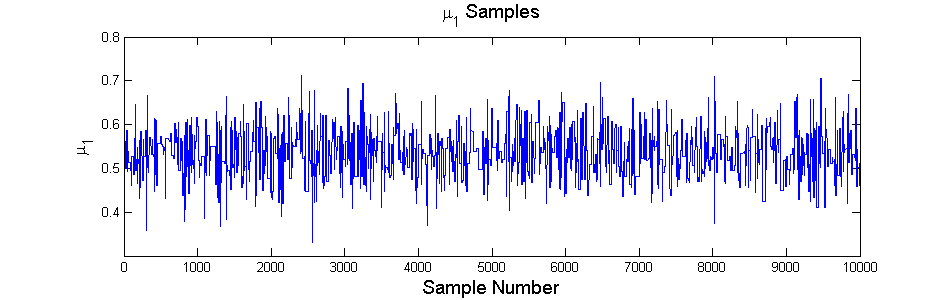
\includegraphics[scale=0.75]{Mu1Samples}\\
\end{center}

Next plot is that of $\mu_1$ v/s $\mu_2.$
\begin{center}
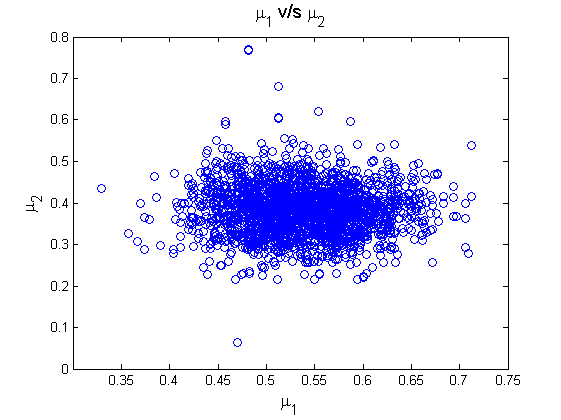
\includegraphics[scale=0.75]{Mu1vsMu2}\\
\end{center}

\noindent {\underline{\textbf{Point and interval estimates of number of days that were weekdays ($k$):}}}\\

$k \rightarrow 72.4366$ [$36 ,97$].\\

\noindent {\underline{\textbf{Probability that proportion of weekends is less than $2/7=0.5579$}}}\\

\pagebreak

\noindent {\underline{\textbf{Point and interval estimates of all parameters:}}}\\
$\mu_1 \rightarrow 0.5403$ [$0.4481  ,  0.6373$].\\
$\sigma_1^2 \rightarrow  1.2155$ [$0.7776 ,   1.8222$].\\
$\mu_2 \rightarrow  0.3831$ [$0.2859   , 0.4805$].\\
$\sigma_2^2 \rightarrow 1.1263$ [$0.3057 ,   2.3891$].\\

\noindent {\underline{\textbf{Point and interval estimates from last time:}}}\\
$\mu_1 \rightarrow 0.4102$ [$0.3037,0.5219$].\\
$\sigma_1^2 \rightarrow  0.8585$ [$0.5750,1.2491$].\\
$\mu_2 \rightarrow  0.1533$ [$0.0462,0.2561$].\\
$\sigma_2^2 \rightarrow 2.4503$ [$1.4273,4.1320$].\\

If we compare our current estimates to estimates from last time we observe that the separation between $\mu_1$ and $\mu_2$ is much smaller. In fact there is a slight overlap in our credible intervals for $\mu_1$ and $\mu_2$ despite using priors such that $\mu_1 > \mu_2.$ This is because this time we have added uncertainty about what type of day it is. 

\pagebreak
\noindent {\Large\underline{\textbf{Appendix:}}}\\
\lstinputlisting{C:/Users/ksp6/Documents/Classes/2013-Fall/STA601-BayesAndModStats/labs/lab9/sta601_ksp6_Lab9.m}

\end{document}